V této kapitole se vrátíme k základní úloze kvantové chemie, tj. k řešení elektronové Schr\"{o}dingerovy rovnice pro danou molekulu. Ukážeme si, jak tuto rovnici můžeme v principu obecně řešit pro atomy a molekuly.  Existují v zásadě tři přístupy k tomuto problému:

\begin{itemize}

\item \textit{Ab initio} metody.  Schr\"{o}dingerovy  rovnici řešíme pomocí hierarchie různě chytrých aproximací (obvykle přitom začínáme Hartreeho-Fockovou metodou) bez dodatečných parametrů. Tyto metody se nazývají \textit{ab initio} (z lat. \uv{\it{od počátku}}, jelikož k výpočtům nevyužíváme než základních fyzikální konstanty jako je hmotnost a náboj elektronu nebo Planckova konstanta. 

\item Semiempirické metody. Tyto metody jsou založeny na principech kvantové mechaniky, některé parametry (typu coulombický či rezonanční integrál) se ale přímo nepočítají, ale nastavují se buď z experimentálních dat nebo z přesnějších \textit{ab initio} výpočtů.

\item Metody založené na teorii funkcionálu hustoty.  Teorie funkcionálu hustoty (DFT, z angl. \textit{Density Functional Theory}) představuje fundamentálně odlišný přístup od předchozích dvou. Není založen na hledání vlnové funkce, ale soustředí na mnohem jednodušší veličinu -- elektronovou hustotu. DFT metoda je často řazena mezi \textit{ab initio} metody, jelikož v principu vede k přesnému řešení a praktická přesnost je taktéž na úrovni \textit{ab initio} metod. Na druhou stranu ale většina DFT metod obsahuje několik empirických parametrů, které se často fitují na experimentální data.    

\end{itemize}

V této kapitole se zaměříme na \textit{ab initio} metody, metody založené na funkcionálu hustoty a semiempirické metody probereme v následujících kapitolách. Nejjednodušší \textit{ab initio} metodou je metoda Hartreeho--Fockova, která již byla stručně představena v kapitolách \ref{kap:viceelektron} a \ref{kap:elstruktmol}
V praxi se dnes používá spíše méně, ale stále slouží jako odrazový můstek pro většinu ostatních přesnějších \textit{ab initio} metod, tudíž si ji zde zopakujeme a probereme hlouběji.

Bude užitečné ujasnit si na začátku notaci užitou v této kapitole, abychom se ve všech těch řeckých písmenech neztratili. Celkovou vlnovou funkci budeme značit symbolem $\psi$,  zatímco molekulové \textbf{spinorbitaly} (MO) budeme značit $\varphi$. Každý MO je součinem \textbf{prostorové části} $\phi$ a \textbf{spinové části} $\alpha$ nebo $\beta$. V rámci aproximace MO-LCAO poté každou prostorovou část MO rozvíjíme do báze \textbf{atomových orbitalů} $\chi_i$. Abychom si ušetřili práci s psaním rovnic, budeme v této kapitole důsledně využívat atomové jednotky. Počet elektronů značíme $N$ a počet jader $K$.

\begin{table}[ht]
\centering
\caption{Základní symboly použité v následujících kapitolách.}
\begin{tabular}{|c|l|c|}
\hline 
\rule[-1ex]{0pt}{2.5ex} Symbol & 	Význam	& Vlastnosti \\ 
\hline 
\rule[-1ex]{0pt}{2.5ex} $\psi$ & Celková el. vln. funkce  & $\psi$ = $det|\phi_1 \phi_2 \cdots \phi_N |$ \\ 
\hline 
\rule[-1ex]{0pt}{2.5ex} $\varphi$ & Molekulový orbital & $\varphi_i=\phi_i \alpha $\\ 
\hline 
\rule[-1ex]{0pt}{2.5ex} $\phi$ & Prostorová část MO & $\phi_i=\sum_{j=1}^N \chi_j $ \\ 
\hline 
\rule[-1ex]{0pt}{2.5ex} $\alpha$, $\beta$  & Spin--orbitaly & \\ 
\hline 
\rule[-0ex]{0pt}{2.5ex} $\chi$ & atomové orbitaly & $\int |\chi|^2 \mathrm{d}\textbf{r} = 1 $ \\
\hline
\end{tabular} 
\label{tab:vlnfunkce}
\end{table}

\subsection{Hartreeho-Fockova metoda}

Zopakujme si nejprve základní teze Hartreeho-Fockovy teorie. Začneme tím, že celkovou vlnovou funkci předpokládáme ve formě Slaterova determinantu (SD)
\begin{equation}
\psi^HF=\frac{1}{\sqrt{N!}}\begin{vmatrix}
\varphi_1(1) & \varphi_1(2) & \cdots & \varphi_1(N) \\
\varphi_2(1) & \varphi_2(2) & \cdots & \varphi_2(N) \\
\vdots & \vdots & \vdots & \vdots \\
\varphi_N(1) & \varphi_N (2) & \cdots & \varphi_N(N)
\end{vmatrix}.
\end{equation}
Jelikož SD má $N!$ členů, kde $N$ je počet elektronů, je třeba použít normalizační faktor $\frac{1}{\sqrt{N!}}$. Vlnová funkce ve tvaru součinu nám říká, že předpokládáme nezávislý pohyb elektronů (v poli jader a ve zprůměrovaném poli ostatních elektronů).

Optimální jednoelektronové vlnové funkce, tj. orbitaly, získáme pomocí variačního principu. Funkcionál energie v rámci metody HF má tvar 
\begin{equation}
E^{HF}=  
\end{equation}

Tento vztah byl odvozen za předpokladu, že jsou molekulové orbitaly ortogonální. Tento požadavek je ryze praktického rázu, ke stejnému výsledku bychom došli i bez něj, ale mnohem obtížněji. Aplikací variačního počtu na předchozí rovnici (více o funkcionálech a variacích si povíme v kapitole o DFT) dostaneme Fockovy rovnice: \textbf{nejsem si jist, zda zde jsou spin orbitaly nebo ne, musim zkontrolovat}
\begin{equation}
\hat{F}\phi_i(1) = \epsilon_i \phi_i 
\label{rov:abinitio:fockrov}  
\end{equation}

kde Fockův operátor $\hat{F}$ má tvar:

\begin{eqnarray}
\hat{F}_i = \sum_{i=1}^{N} \hat{h}_i+\sum_{j\neq i} \hat{J}_j - \delta(s_i,s_j) \hat{K}_j \\ \label{rov:abinitio:fockoper}
\hat{h}_i = -\frac{1}{2}\Delta_i - \sum_{A}\frac{Z_A}{r_{iA}}
\hat{J}_j=\int \frac{|\varphi |^2}{r_{ij}}\mathrm{d}\textbf{r}_j \\
\hat{K}_{ij} = \int \frac{\phi_j^*(\mathbf{r}_j)\phi_i(\mathbf{r}_i)}{r_{ij}}\mathrm{d}\textbf{r}_j
\end{eqnarray}

V členu XXX rozpoznáváme kinetickou energii jednoho elektronu a přitažlivou interakci mezi i-tým elektronem a jádrem A. Člen se sumačním znaménkem popisuje interakci elektronu s ostatními elektrony, obsahuje coulombovskou člen XXX a výměnný člen XXXXX.


Fockovy rovnice jsou složité integro-diferencíální rovnice pro neznámé funkce $\phi_i$,
což jsou naše hledané molekulové orbitaly.
Tyto rovnice typicky řešíme rozvojem molekulových orbitalů do báze orbitalů atomových
\begin{equation}
\phi=\sum_{i=1}^K c_i \chi_i ,
\end{equation}
čímž problém rapidně zjednodušíme, jelikož nyní nehledáme funkce, ale jen číselné koeficienty $c_i$.
Výsledné rovnice (pro případ uzavřené slupky) se nazývají Roothanovy, což jsou následující algebraické rovnice
\begin{equation}
ROOTHAN
\end{equation}


Jelikož molekuly jsou složeny z atomů, vhodnou bází jsou atomové orbitaly.
Dnes se již téměř výhradně používají Gaussovy funkce, o kterých již byla řeč v kapitole \ref{sec:AObasis}.
Pokud bychom použili nekonečně velkou bázi, získali bychom tzv. Hartreeho--Fockovu limitu a naše MO by měli nejlepší možný tvar. Tato limita ale \textbf{není} přesné řešení elektronové Schr\"{o}dingerovy rovnice!
Předpokládali jsme totiž vlnovou funkci ve tvaru Slaterova determinantu. Tato vlnová funkce ale trpí principiálními defekty. V přesné vlnové funkci by se nám třeba nikdy nemohlo stát, že bychom nalezli dva elektrony na jednom místě, takovéto uspořádání by totiž dle Coulombova zákona mělo nekonečnou energii.
Na tomto místě je dobré si uvědomit, že celý koncept molekulových orbitalů, na které jsou chemici již tak zvyklí, je založen na HF teorii, a je tudíž pouze aproximací. Jakmile se budeme snažit dosáhnout přesnějších výsledků, začne se nám úhledný obrázek elektronů sedících v molekulových orbitalech rozpadat.

Jelikož je HF metoda metodou variační, je energie HF limity vyšší než skutečná energie získaná přesným řešení nerelativistické Schr\"{o}dingerovy rovnice.
Rozdíl mezi těmito dvěma metodami se nazývá korelační energie
\begin{equation}
E_{kor}=E_{el} - E^{HF}
\end{equation}
a je důsledkem toho, že jsme zanedbali okamžitou mezi-elektronovou repulzi.

%OBRAZEK KORELACNI ENERGIE ATP

%TODO rict neco o Fermiho dire????

Pro výpočet korelační energie je třeba použít pokročilejších metod, které popíšeme v následujících kapitolách.

\subsection{Poruchový přístup: M\o llerova-Plessetova metoda}
HF metoda popisuje nezávisle se pohybující elektrony. Skutečné elektrony se úplně nezávisle nepohybují, jejich pohyb je korelován. Rozdíl mezi HF elektrony a skutečnými elektrony ale obvykle není příliš velký, takže bychom mohli použít poruchovou teorii.  Existují různé cesty k poruchovému řešení elektronové Schr\"{o}dingerovy rovnice, nejčastěji se setkáváme se metodou, kterou zavedli dánští badatelé M\o ller a Plesset.

V poruchové metodě je třeba nejprve najít problém, který jsme schopni řešit a který je dostatečně blízko přesnému řešení. K tomuto zde využijeme HF teorie. Nyní je třeba vymyslet, jaký je vlastně hamiltonián HF metody, abychom poté podle rovnice \ref{rov:approx:ham} mohli skutečný hamiltonián rozdělit na poruchu a HF Hamiltonián.
\begin{equation}
\hat{H}^{\prime}_{MP}=\hat{H}_{el} - \hat{H}^{(0)}_{HF}
\end{equation}

Jelikož Fockovy rovnice \ref{rov:abinitio:fockrov} jsou rovnicemi jednoelektronovými, bude se celkový hamiltonián skládat ze součtu jednoelektronových Fockových operátorů \ref{rov:abinitio:fockoper}
\begin{equation}
\hat{H}^{(0)}_{HF}= \sum_{i=1}^N \hat{F}_i
\label{rov:abinitio:hfham}
\end{equation}
Energie tohoto hamiltoniánu je potom rovna součtu orbitálních energií
\begin{equation}
E^{(0)}_{HF}=\sum_{i=1}^N \epsilon_i .
\end{equation}
Pozor, toto není HF energie! V součtu orbitálních energií jsou mezielektronové interakce započteny dvakrát. Nyní můžeme přejít k definici naší poruchy odečtením rovnice \eqref{rov:abinitio:hfham} od elektronového hamiltoniánu. Jednoelektronové členy se vyruší a vyjde nám
\begin{equation}
\hat{H}^{\prime}_{MP}=\hat{H}_{el}-\hat{H}^{(0)}_{HF}= \frac{1}{2}\sum_{j\neq i} \frac{1}{\textbf{r}_{ij}} - \left(\sum_{j\neq i} \hat{J}_j - \delta(s_i,s_j) \hat{K}_j \right) .
\end{equation}
Vidíme, že porucha je dána rozdílem mezi coulombickým členem a efektivním polem elektronů v HF teorii.

Zkusme si nyní podle vzorce \eqref{rov:PorusenaEnergie} vypočítat energii do prvního řádu. Platí, že
\begin{equation}
E_1=E^{(0)}_{HF} + E^{(1)}= \sum_{i=1}^N \epsilon_i - 
\end{equation}
To jsme se daleko nedostali! Porucha v prvním řádu nám ve výsledku dá původní HF energii.
Užitečná je tedy až porucha druhého řádu, pro kterou ze vzorce \eqref{rov:aprox:energiePT2} platí:
\begin{equation}
E^{MP2} = E^{HF} + \sum_m \frac{\left < \psi^{(0)}_{HF}|\hat{H}^{\prime}_{MP}|\psi_n^{(0)} \right >}{E_{HF}^{(0)}-E_m^{(0)}}\psi_m^{(0)}.
\end{equation}

Vypadá to, že budeme muset počítat spoustu maticových elementů mezi základním stavem a všemi excitovanými Slaterovými determinanty (o těch si více povíme v další podkapitole). Naštěstí se dá ukázat (díky tzv. Brillouinovu\footnote{Toto jméno vysloví opravdu jen zkušení frankofilové.} teorému a Slaterovým-Condonovým pravidlům), že většina z nich bude nulová a přispívat budou jen dvojitě-excitované determinanty, které zde zjednodušeně značíme $\psi_{ij}^{rs}$ (excitujeme dva elektrony z orbitalů $i$ a $j$ do orbitalů $r$ a $s$). Výsledný vzorec tudíž bude
\begin{equation}
E^{MP2}=\sum_{ij} \sum_{rs} \frac{\left < \psi_0 | \hat{H}^{\prime}_{MP} | \psi_{ij}^{rs} \right > }{\epsilon_r+\epsilon_s-\epsilon_i-\epsilon_j} .
\end{equation}
Metoda zahrnující příspěvky do druhého řádu teorie poruch má zkratku MP2 a je jednou s nejvíce užívaných metod na výpočet korelační energie. Mohli bychom pokračovat a odvodit vzorce pro vyšší řády a dostali bychom pak metody MP3, MP4 atd. 
Metoda MP3 nepřináší výrazné zlepšení oproti MP2 a tudíž není využívána. Metoda MP4 je velmi přesná, ale také velmi výpočetně náročná. Ani ona se v dnešní dobře příliš nevyužívá, pro velkou přesnost je totiž výhodnější použít metody spřažených klastrů, o kterých bude řeč za chvíli.


\subsection{Metoda konfigurační interakce}

Alternativní cestu ke korelační energii nabízí variační princip. Dá se ukázat, že množina všech Slaterových determinantů, které můžeme vytvořit z HF molekulových orbitalů nahrazením některých obsazených molekulových orbitalů orbitaly v základním stavu neobsazenými, vytváří úplný soubor funkcí. Můžeme tak do něj rozvinout přesnou vlnovou funkci 
\begin{equation}
\psi_{CI}=C_0\psi_0+\sum_a\sum_m C_a^m\psi_a^m+\sum C_{ab}^{mn}\psi_{ab}^{mn}+\dots
\label{rov:CIrozvoj}
\end{equation}
kde první člen je Slaterův determinant základního stavu a další členy odpovídající determinantům, kde jsme excitovali jeden nebo více elektronů z obsazeného do neobsazeného orbitalu (viz obrázek \ref{obr:abinitio:ci}). Druhý člen odpovídá mono-excitacím (obr. \ref{obr:abinitio:ci}A), třetí člen odpovídá bi-excitacím (obrázek \ref{obr:abinitio:ci}B) atp. Jednotlivým Slaterovým determinantům můžeme také říkat konfigurace, odtud název metody konfigurační interakce (CI, z angl. \textbf{Configuration Interaction}).

\begin{figure}
\centering
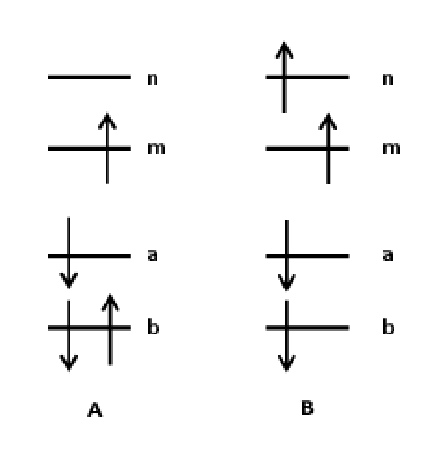
\includegraphics[scale=1]{CIkonfigurace.eps}
\caption[Excitované Slaterovy determinanty]{Ukázka mono-excitovaných (\textbf{A}) a bi-excitovaných (\textbf{B}) Slaterových determinantů.}
\label{obr:abinitio:ci}
\end{figure}

Jak nyní určíme koeficienty $C$ (pozor, neplést s koeficienty $c$ v HF metodě)? Opět pomocí variačního principu. Jelikož vlnová funkce na těchto koeficientech závisí lineárně, aplikací variačního principu dostaneme již mnohokrát zmíněné sekulární rovnice
\begin{eqnarray}
\mathbb{H}\mathbf{c}=E\mathbf{c} \nonumber \\
\sum_j (H_ij-E_i\delta_{ij})c_i=0 \quad \forall i
\end{eqnarray}
kde maticové elementy $H_{ij}$ představují integrály mezi Slaterovými determinanty

 
XXXXXX

Výsledné matice $\mathbb{H}$ mohou být často obrovské (rozměr milion x milion není vůbec šokující), ale existují efektivní metody výpočetní lineární algebry, které si s nimi dokáží poradit.

Pokud bychom použili nekonečnou bázi AO a zahrnuli všechny možné Slaterovy determinanty (kterých by bylo taktéž nekonečné mnoho), dostali bychom přesné řešení Schr\"{o}dingerovy rovnice. V praxi ale musíme použít bázi konečnou, máme tedy i konečný počet molekulových orbitalů. Pokud v rámci této báze budeme uvažovat všechny možné Slaterovy determinanty, mluvíme o metodě úplné konfigurační interakce (FCI, z angl.\textit{Full Configuration Interaction}). Zvětšováním báze se metoda FCI může libovolně přiblížit přesnému řešení. Metoda FCI je ale extrémně výpočetně náročná (náročnost roste exponenciálně s počtem orbitalů) a lze ji tedy použít pouze pro malé molekuly s malou bází.

Pro praktické výpočty tedy musíme počet excitací omezit. Pokud se omezíme pouze jednonásobné a dvojnásobné excitace, získáme metodu CISD (z angl. \textit{Configuration Interaction Singles}\& \textit{Doubles}), která byla v minulosti hojně využívána.

Dnes se metody konfigurační interakce užívají méně, jelikož mají některé nevýhody oproti jiným metodám. 
\begin{itemize}
\item Metoda FCI je sice přesná, ale v praxi díky exponenciálnímu škálování nepoužitelná.
\item Rozvoj \ref{rov:CIrozvoj} konverguje velmi pomalu. Pro dobrou přesnost bychom chtěli minimálně čtyřnásobné-excitace.
\item Pokud použijeme konečný rozvoj \ref{rov:CIrozvoj}, tak výsledná metoda nemá správnou závislost na velikosti systému (v žargonu kvantových chemiků, metoda není \uv{size konsistentní}). Co tento pojem znamená? Zjednodušeně řečeno, pokud metoda není \uv{size konsistentní}, tak její přesnost bude záviset na velikosti systému. Pro malou molekulu můžeme například metodou CISD zachytit přes 90 \% korelační energie, ale pro větší molekulu mnohem méně. Pro \uv{size konsistentní} metodu by mělo platit, že energie dvou nekonečně vzdálených molekul by měl být přesně roven dvojnásobku energie jedné molekuly. Na příkladu dvou atomů helia lze ale snadno ukázat, že toto pro metodu CISD není splněno. Pro jeden atom He totiž metoda CISD odpovídá metodě FCI, jelikož máme pouze dva elektrony, které můžeme excitovat. Pro dva nekonečně vzdálené atomy helia již ale toto neplatí, jelikož máme už čtyři elektrony a některé Slaterovy determinanty tudíž nebudou v CISD metodě zahrnuty. 
%(\textbf{obrázek? PSnote: Ano})
Metoda MP2 či metoda spřažených klastrů \uv{size konsistentní} jsou, metoda CI naopak nikoliv. 
\end{itemize}


\subsection{Metody spřažených klastrů}
Metody spřažených klastrů (CC, z angl.\textit{Coupled Cluster}) nesou od svého počátku českou stopu. Tyto metody totiž použil v kontextu kvantové chemie poprvé Jiří Čížek a později také Josef Paldus. Metoda konfigurační interakce je založena na mazaném přeskládání rozvoj typu CI. Klíčovým pojmem v této metodě jsou takzvané excitační operátory. Například operátor $\hat{T}_1$ působí na vlnovou funkci základního stavu jako
\begin{eqnarray}
\hat{T}_1\psi_0=\sum^N_{a=1}\sum_{m=n+1}^\infty t_a^m\psi_a^m , 
\end{eqnarray}
tj. generuje lineární kombinaci mono-excitovaných konfigurací.  Tento operátor obsahuje neurčené koeficienty $t_a^m$ popisujících zapojení jednotlivých excitovaných konfigurací do celkové vlnové funkce. Obdobně operátor $\hat{T}_2$ 
\begin{eqnarray}
\hat{T}_2\psi_0=\sum_{a=1}^N \sum_{b\neq a}^N\sum_{m=N+1}^\infty \sum_{n=N+1}^\infty t_{ab}^{mn}\psi_{ab}^{mn}
\end{eqnarray}
generuje lineární kombinaci  bi-excitovaných konfigurací atp. Celkový excitační operátor píšeme jako
\begin{eqnarray}
\hat{T}=\hat{T}_1+\hat{T}_2+\cdots \hat{T}_N.
\end{eqnarray}

Vlnovou funkci v rámci metody spřažených klastrů zapisujeme v poněkud neobvyklém tvaru
\begin{eqnarray}
\psi^{CC} = e^{\hat{T}} \psi_0 ,  \\
\end{eqnarray}
kde $\psi_0$ je referenční funkce, většinou z metody HF. Zde se poprvé setkáváme s pojmem exponenciály operátoru. Není třeba se jej leknout, jen si musíme uvědomit, jak je vlastně definována normální exponenciální funkce $e^x$. Exponenciální funkci čísla můžeme definovat pomocí Taylorova rozvoje
\begin{equation}
e^x=\sum_{i=1}^\infty \frac{x^n}{n!} .
\end{equation}
Tu samou definici nyní můžeme snadno aplikovat i na operátory, musíme jen vědět, jak operátory umocňovat.
To jsme si ale řekli již v kapitole \ref{kap:OperaceSOperatory}. Operátor umocněný na $n$-tou prostě znamená, že jej aplikujeme $n$-krát za sebou na tu samou funkci. Exponenciela excitačního operátoru tedy vyjde jako 
\begin{equation}
e^{\hat{T}} = 1+\hat{T}+\frac{\hat{T}^2}{2}+\cdots.
\end{equation}
Díky vlastnostem excitačního operátoru je tato řada konečná, neboť molekula má pouze konečný počet elektronů, které lze excitovat.

Jaká je vlastně výhoda takto složitého zápisu?
Pokud použijeme úplný excitační operátor, tak dojdeme k exaktnímu řešení stejně jako metoda FCI. Budeme ale potřebovat stejné množství parametrů, ať už je nazýváme rozvojovými koeficienty (v metodě CI) nebo amplitudami (v metodě CC).
Výhody se ale objeví, když excitační operátor začneme ořezávat. Když například vezmeme v potaz pouze mono- a double-excitace, dostaneme metodu CCSD  (z angl. \textit{Coupled Cluster Singles Doubles}).
Na rozdíl od metody CISD je ovšem CCSD \uv{size-konzistentní} a navíc dostaneme větší podíl korelační energie.
To je dáno právě speciálním tvarem CC vlnové funkce, díky kterému i na úrovni CCSD dostaneme například i částečný příspěvek čtyřnásobných excitací, jelikož v exponenciální řadě je přítomen operátor $\hat{T}_2^2$. K tomu nám ale stačí stejný počet parametrů jako v metodě CISD.

Vzorec pro energii v rámci metod typu CC je složitější, poněkud náročnější jsou také pracovní rovnice této metody určující koeficienty $t$ excitačního operátoru. Metody spřažených klastrů jsou stejně jako poruchové metody size-konzistnentní a obdobně nejsou variační. Ukazuje se ale, že v praxi je právě správná závislost na velikosti systému důležitější, a proto se metody konfigurační interakce dnes používají méně často než poruchové metody a metody spřažených klastrů.

Jak jsme si již řekli v předchozí podkapitole, metody konfigurační interakce konvergují dosti pomalu k přesnému řešení. Tvar vlnové funkce v metodě spřažených klastrů tuto konvergenci značně urychluje. Už se zahrnutím trojitých excitací dostáváme výsledky s chemickou přesností (tzn. relativní energie s přesností 1\,kcal/mol což je zhruba 4\,kJ/mol.
Metoda CCSD(T) je v současné době považována za \uv{zlatý standard} kvantové chemie. V metodě CCSD(T) jsou trojité excitace zahrnuty v rámci poruchového počtu. Výpočetní náročnost této metody dovoluje na současné úrovni popsání molekul s 10-50
%TODODH: jaky je tu ten rozsah?
atomy. Užitím speciálních technik lineárního škálování lze ale toto použití značně rozšířit, nedávno tak byla tato metoda aplikována na malou molekulu proteinu obsahující stovky atomů. 

\subsection{Multireferenční metody}

Všechny metody, které jsme probrali výše, vychází z Hartreeho-Fockovy metody. Předpokládají, že popis molekuly pomocí jednoho Slaterova determinantu je v zásadě v pořádku, jenom je potřeba udělat menší \uv{facelift}. Někdy je ale popis jediným Slaterovým determinantem z gruntu špatně. Kupodivu se se selháním Hartreeho-Fockovy metody můžeme setkat i v jednoduchých situacích Uvažme molekulu vodíku H$_2$ v základním stavu. Na Obr. \ref{obr:multiref} je ukázán diagram orbitálních energií pro rovnovážnou geometrii a pro disociovanou strukturu. Uvažme první případ. Zde bez potíží umístíme dva elektrony do nejnižšího orbitalu XXX, což odpovídá Slaterovu determinantu

\begin{equation}
\Psi (1,2)=\frac{1}{\sqrt{2}}
\begin{vmatrix}
\sigma_g(1)\alpha (1) & \sigma_g(2)\alpha (2) \\
\sigma_g(2)\beta (2) & \sigma_g(2)\beta (2)
\end{vmatrix}
=\frac{1}{\sqrt{2}}\sigma_g(1)\sigma_g(2)(\alpha (1)\beta (2)-\alpha (2)\beta (1))
\end{equation}

Jenomže pro disociovanou strukturu (což je v tomto  případě triviálně řešitelný problém metodou separace proměnných s řešením XXXX a XXXXX)teď nevíme, jaký orbital vlastně dosadit do Slaterova determinantu XXX. Vazebný nebo antivazebný? Vždyť mají oba stejnou energii. V nejjednodušším případě, kdy 

XXXXXXX

\noindent získáme vlnovou funkci


XXXXXXXX


\noindent První dva členy zde odpovídají (správně) kovalentní struktuře, ale druhé dva členy popisují ionty, H+...H- a H-...H+. Tomu bude odpovídat energie, která bude z poloviny dána jako neutrálními atomu a z poloviny ionty (voiz Obr. XXX). Správná vlnová funkce je dána rozvojem


XXXXXXXXXXXXXXXXXXXXXX



\noindent je tedy vidět, že v případě rozštěpení chemické vazby za vzniku bi-radikálové struktury je potřeba použít více než jeden Slaterův determinant. Metoda HF kvalitativně selhává. Ŕešením je použít velmi omezený rozvoj typu konfigurační interakce

XXXXX

\noindent do kterého zahrneme pouze excitace z orbitalů v blízkosti nejvyššího obsazeného molekulového orbitalu HOMO (z angl. \textit{Highest Occupied Molecular Orbital}) a z nejnižšího neobsazeného molekulového orbitalu LUMO (a angl. \textit{Lowest Unoccupied Molecular Orbital}). Tuto množinu orbitalů, ze kterých a do kterých excitujeme, nazýváme aktivním prostorem. Tato metoda má zkratku CASSCF (z angl. \textit{Complete Active Space-Slef Consistent Field}). 


Metoda CASSCF pokrývá tu část korelační energie, která souvisí s principiální nedostatečností jednoho Slaterova determinantu pro popis molekuly, mluvíme o tzv. statické korelaci. I v metodě CASSCF s konečným aktivním prostorem je ale nesprávně popsána okamžitá interakce mezi elektrony, tj. tzv. dynamická korelace.\footnote{Dělení korelační energie na statickou a dynamickou je poněkud umělé a difúzní.} Dynamickou korelaci pak můžeme dodat kupříkladu pomocí poruchové teorie aplikované na referenční vlnovou funkci z metody CASSCF (v případě poruchové teorie druhého řádu pak dostaneme často užívanou metodu CASPT2) nebo pomoci metody konfigurační interakce (zde dostaneme metodu multireferenční konfigurační interakce, MRCI). Obecně mluvíme o multi-referenčních metodách.

Disociace vazby za vzniku biradikálů není ale jediná situace, pro kterou je metoda HF nedostatečná. Jiným takovým případem jsou excitované stavy molekul. I kdyby byl základní a excitovaný stav popsán kvalitně jedním Slaterovým determinantem, půjde o jiný Slaterův determinant pro každý ze stavů. Pro konzistentní popis obou stavů najednou (třeba při výpočtech excitačních energií) je tudíž žádoucí opět použít rozvoj do více Slaterových determinantů. S multireferenčními metodami se proto často setkáme ve spektroskopii a fotochemii. 

